\documentclass{report}

%!Tex Root = ../main.tex

% ┌────────────┐
% │ Formatting │
% └────────────┘
\usepackage[english]{babel}
\usepackage[export]{adjustbox} % use c, l, r for images
\usepackage{csquotes}
\usepackage[parfill]{parskip}
% \usepackage[margin=1.5cm, headheight=0cm]{geometry}
\usepackage{geometry}
\usepackage{titlesec}
\usepackage{fix-cm}
\usepackage[usetoc]{titleref}

% ┌───────────────────┐
% │ Table of Contents │
% └───────────────────┘
\usepackage{titletoc}
\usepackage[nottoc]{tocbibind}

% ┌──────┐
% │ Math │
% └──────┘
\usepackage{amssymb} % for black triangleright, https://tex.stackexchange.com/questions/570303/use-blacktriangleright-as-itemize-label
\usepackage{amsmath}
\usepackage{mathtools} % for \mathclap and 
\usepackage{breqn}

% ┌────────┐
% │ Tables │
% └────────┘
\usepackage{tabularray}
 % \UseTblrLibrary{diagbox}

% ┌────────┐
% │ Images │
% └────────┘
\usepackage{graphicx}
\usepackage{float} % for the letter H
% \graphicspath{figures/}
\usepackage[labelfont={color=PrimaryColor, bf}, textfont={it}]{caption}
\usepackage{subcaption}

% ┌──────────┐
% │ Diagrams │
% └──────────┘
\usepackage{tikz}
\usetikzlibrary{mindmap, shadows, backgrounds} % , calc
\usepackage{tikzit}
\usepackage{tikz}
\usetikzlibrary{backgrounds}
\usetikzlibrary{arrows}
\usetikzlibrary{shapes,shapes.geometric,shapes.misc}

% this style is applied by default to any tikzpicture included via \tikzfig
\tikzstyle{tikzfig}=[scale=0.5]

% these are dummy properties used by TikZiT, but ignored by LaTex
\pgfkeys{/tikz/tikzit fill/.initial=0}
\pgfkeys{/tikz/tikzit draw/.initial=0}
\pgfkeys{/tikz/tikzit shape/.initial=0}
\pgfkeys{/tikz/tikzit category/.initial=0}

% standard layers used in .tikz files
\pgfdeclarelayer{edgelayer}
\pgfdeclarelayer{nodelayer}
\pgfsetlayers{background,edgelayer,nodelayer,main}

% style for blank nodes
\tikzstyle{none}=[inner sep=0mm]

% include a .tikz file
\newcommand{\tikzfig}[1]{%
{\tikzstyle{every picture}=[tikzfig]
\IfFileExists{#1.tikz}
  {\input{#1.tikz}}
  {%
    \IfFileExists{./figures/#1.tikz}
      {\input{./figures/#1.tikz}}
      {\tikz{\node[draw=red,font=\color{red},fill=red!10!white] {\textit{#1}};}}%
  }}%
}

% the same as \tikzfig, but in a {center} environment
\newcommand{\ctikzfig}[1]{%
\begin{center}\rm
  \tikzfig{#1}
\end{center}}

% fix strange self-loops, which are PGF/TikZ default
\tikzstyle{every loop}=[]


% ┌────────┐
% │ Citing │
% └────────┘
% \usepackage[style=numeric]{biblatex}
% \addbibresource{./Missing_Semester.bib}

% ┌─────────┐
% │ Itemize │
% └─────────┘
\usepackage{enumitem}

% ┌────────────────────┐
% │ Code hightligthing │
% └────────────────────┘
% \usepackage{minted}

% ┌───────────────────┐
% │ Header and Footer │
% └───────────────────┘
\usepackage{fancyhdr}

% ┌────────────────────────┐
% │ Latex Programming Help │
% └────────────────────────┘
\usepackage{etoolbox}
\usepackage{xparse}
% https://tex.stackexchange.com/questions/358292/creating-a-subcounter-to-a-counter-i-created
\usepackage{chngcntr}
\usepackage{totcount}

% ┌───────┐
% │ Boxes │
% └───────┘
\usepackage{xcolor}
\usepackage{tcolorbox}
\tcbuselibrary{skins}
\tcbuselibrary{theorems}
\usetikzlibrary{patterns}
\tcbuselibrary{breakable}
\usepackage[bold=1]{xfakebold}
\tcbuselibrary{minted}

% ┌────────┐
% │ Colors │
% └────────┘
\definecolor{PrimaryColor}{HTML}{344A9A}
\definecolor{PrimaryColorDimmed}{HTML}{A4B1E0}
% \definecolor{SecondaryColor}{HTML}{006BB6}
% \definecolor{SecondaryColorDimmed}{HTML}{E5F0F8}
\definecolor{SwitchColor}{named}{PrimaryColor}
\colorlet{BoxColor}{gray!10!white}


% ┌───────┐
% │ Links │
% └───────┘
% \usepackage[allbordercolors=PrimaryColor, pdfborder={0 0 .2}]{hyperref}
\usepackage[colorlinks=true, allcolors=PrimaryColor]{hyperref}

% ┌──────────────┐
% │ Pseudo Code  │
% └──────────────┘
\usepackage{pseudo}

% ┌────────────┐
% │ Misc Tools │
% └────────────┘
% \usepackage{lipsum}

% ┌───────┐
% │ Fonts │
% └───────┘
\usepackage{fontspec}

%!Tex Root = ../main.tex

% ┌────────────┐
% │ Linebreaks │
% └────────────┘
% https://norwied.wordpress.com/2012/07/10/how-to-break-long-urls-in-bibtex/
\def\UrlBreaks{\do\/\do-\do\&\do.\do:}

% ┌───────┐
% │ Boxes │
% └───────┘
\newtcolorbox{titlebox}[1]{colback=PrimaryColorDimmed,colframe=PrimaryColor,arc=0.2cm,boxrule=0cm,frame hidden,left=0cm,right=0cm,top=0.1cm,toptitle=0.2cm,bottom=0.1cm,bottomtitle=0.2cm,boxsep=0cm,fonttitle=\bfseries,title={#1}}

% https://tex.stackexchange.com/questions/433256/inline-tcolorbox-with-rotated-title
\DeclareTotalTCBox{\points}{ s m }
{colback=PrimaryColorDimmed,boxrule=0cm,frame hidden,nobeforeafter,tcbox raise base,top=0mm,bottom=0mm,
	right=0mm,left=0mm,arc=0.1cm,boxsep=0.1cm}
{#2}

\DeclareTotalTCBox{\inlinebox}{ s m }
{verbatim,colback=PrimaryColorDimmed,colframe=PrimaryColor,nobeforeafter,tcbox raise base,top=0mm,bottom=0mm,
	right=0mm,left=0mm,arc=0.1cm,boxsep=0.1cm}
{\IfBooleanTF{#1}%
	{\textcolor{PrimaryColor}{\setBold >\enspace\ignorespaces}#2}%
	{#2}}


% \newtcbox{\inlineboxtwo}{capture=minipage,tcbox raise base,breakable,colback=PrimaryColorDimmed,colframe=PrimaryColor,nobeforeafter,top=0mm,bottom=0mm,
% 	right=0mm,left=0mm,arc=0.1cm,boxsep=0.1cm,fontupper=\ttfamily}

\DeclareTotalTCBox{\key}{ m }
{verbatim,colback=PrimaryColorDimmed,colframe=PrimaryColor,nobeforeafter,tcbox raise base,top=0mm,bottom=0mm,
	right=0mm,left=0mm,arc=0.1cm,boxsep=0.1cm}
{$\mathtt{#1}$}

\newtcolorbox{sidenote}{enhanced,boxrule=0cm,frame hidden,arc=0.2cm,title=Sidenote,attach boxed title to top text left={yshift=-0.2cm},colback=PrimaryColorDimmed,boxed title style={boxrule=0cm,frame hidden,colback=PrimaryColor,arc=0.1cm},fonttitle=\bfseries,
	after title={\hspace{0.2cm}
\includegraphics[height=3mm]{./figures/lupe.png}}
}
% drop fuzzy shadow,

% https://tex.stackexchange.com/questions/210928/tcolorbox-how-do-i-align-on-the-baseline-of-the-title
\newtcblisting{terminal}{
	enhanced,box align=top,colframe=PrimaryColor,colback=PrimaryColorDimmed,hbox,arc=0.2cm,bottom=0.1cm,top=0.1cm,left=0.1cm,right=0.1cm,boxrule=0.05cm,listing only,minted language=text,listing engine=minted,minted options={escapeinside=||,autogobble}
}

\newtcblisting{terminal2}{
	enhanced,box align=top,colframe=PrimaryColor,colback=PrimaryColorDimmed,hbox,arc=0.2cm,bottom=0.1cm,top=0.1cm,left=0.1cm,right=0.1cm,boxrule=0.05cm,listing only,minted language=text,listing engine=minted,minted options={escapeinside=!!,autogobble}
}

\DeclareTCBInputListing{\file}{o m}{
	listing file={#2},enhanced,colframe=PrimaryColor,colback=PrimaryColorDimmed,hbox,fonttitle=\bfseries\tiny,halign title=center,arc=0.2cm,boxrule=0.05cm,bottom=0.1cm,top=0.1cm,left=0.1cm,right=0.1cm,listing only,listing engine=minted,#1}

\DeclareTCBListing{dfile}{o}{
	enhanced,colframe=PrimaryColor,colback=PrimaryColorDimmed,hbox,fonttitle=\bfseries\tiny,halign title=center,arc=0.2cm,boxrule=0.05cm,bottom=0.2cm,top=0.1cm,left=0.1cm,right=0.1cm,listing only,listing engine=minted,#1}

% https://tex.stackexchange.com/questions/593218/nested-inline-math-for-new-command-with-argument
\newcommand{\prompt}{\textcolor{PrimaryColor}{\setBold >\;\ignorespaces}}

\DeclareTCBInputListing{\codebox}{ s o m }{listing file={#3},
	enhanced,colframe=PrimaryColor,colback=BoxColor,IfBooleanTF={#1}{colframe=SecondaryColor}{colframe=PrimaryColor},fonttitle=\bfseries\small,#2,listing only,halign title=center,drop fuzzy shadow,arc=0,2cm,boxrule=0.05cm,bottom=0.1cm,top=0.1cm,left=0.1cm,right=0.1cm,listing engine=minted}
% , sharpish corners

\DeclareTCBListing{dcodebox}{ s o }{
	enhanced,colframe=PrimaryColor,IfBooleanTF={#1}{colframe=SecondaryColor,colback=SecondaryColorDimmed}{colframe=PrimaryColor,colback=PrimaryColorDimmed},hbox,fonttitle=\bfseries\small,#2,listing only,halign title=center,drop fuzzy shadow,arc=0.2cm,boxrule=0.05cm,bottom=0.1cm,top=0.1cm,left=0.1cm,right=0.1cm,listing engine=minted}
% , sharpish corners

\DeclareTCBInputListing{\file}{o m}{
	listing file={#2},enhanced,colframe=PrimaryColor,colback=PrimaryColorDimmed,hbox,,fonttitle=\bfseries,halign title=center,arc=0.2cm,bottom=0.2cm,top=0.1cm,left=0.1cm,right=0.1cm,boxrule=0.5mm,listing only,listing engine=minted,#1}

\DeclareTCBListing{dfile}{o}{
	enhanced,colframe=PrimaryColor,colback=PrimaryColorDimmed,hbox,,fonttitle=\bfseries,halign title=center,arc=0.2cm,bottom=0.2cm,top=0.1cm,left=0.1cm,right=0.1cm,boxrule=0.5mm,listing only,listing engine=minted,#1}

\newtcbinputlisting{\numberedcodebox}[2][]{
	listing file={#2}, enhanced, colframe=PrimaryColor,colback=BoxColor,fonttitle=\bfseries\small,#1,listing only,halign title=center,arc=0.2cm,boxrule=0.05cm,bottom=0.1cm,top=0.1cm,left=0.5cm,right=0.1cm,listing engine=minted,overlay={\begin{tcbclipinterior}\fill[PrimaryColorDimmed] (frame.south west) rectangle ([xshift=0.5cm]frame.north west);\end{tcbclipinterior}}
}

\newtcblisting{dnumberedcodebox}[1][]{
	enhanced, colframe=PrimaryColor,colback=PrimaryColorDimmed,fonttitle=\bfseries\tiny,#1,listing only,halign title=center,arc=0.2cm,boxrule=0.05cm,bottom=0.1cm,top=0.1cm,left=0.5cm,right=0.1cm,listing engine=minted,overlay={\begin{tcbclipinterior}\fill[PrimaryColor] (frame.south west) rectangle ([xshift=0.5cm]frame.north west);\end{tcbclipinterior}}
}

% https://tex.stackexchange.com/questions/585582/inside-of-a-newtcbinputlisting-how-can-i-change-the-color-of-the-line-number-as
\renewcommand{\theFancyVerbLine}{\sffamily
	\textcolor{white}{\tiny
		\oldstylenums{\arabic{FancyVerbLine}}}}

% ┌──────────────┐
% │ Bibliography │
% └──────────────┘
% \defbibenvironment{bibliography}
% {\itemize}
% {\enditemize}
% {\item}

% ┌──────────┐
% │ Commands │
% └──────────┘
\newtotcounter{exercisecounter}
\newtotcounter{exercisecounterdec}
\setcounter{exercisecounter}{1}
\newtotcounter{points}
\setcounter{points}{0}
\NewDocumentCommand\exercise{ o o }{
	\vspace{0.5cm}
	\IfValueTF{#1}
	{\textcolor{PrimaryColor}{\bfseries Exercise \theexercisecounter :} #1}
	{\textcolor{PrimaryColor}{\bfseries Exercise \theexercisecounter}}
	\stepcounter{exercisecounter}
	\IfValueT{#2}{
		\hfill\raggedleft\points{\qquad/#2 Subexercises}\ignorespaces\raggedright
		\addtocounter{points}{#2}
	}
}

% ┌──────────────────┐
% │ Case distinction │
% └──────────────────┘
% \newtoggle{whatever}
% \toggletrue{whatever}
% \togglefalse{whatever}
% \newcommand{\lpathx}[1]{\iftoggle{absolute}{/home/areo/Documents/Studium/Summaries/x/}{./}#1}

%!Tex Root = ../main.tex

% ┌────────────┐
% │ Formatting │
% └────────────┘
\setlength{\parskip}{0.4cm} % space between paragraphs, https://latexref.xyz/bs-par.html
\setlength\belowcaptionskip{-0.5cm} % https://stackoverflow.com/questions/2685152/gap-after-table-in-latex
% \mathversion{bold} % math formulas bold


% ┌───────────────────────┐
% │ Chapters and Sections │
% └───────────────────────┘
\titleformat{\chapter}[hang]
{\color{PrimaryColor}\normalfont\huge\bfseries}{\thechapter}{0.5cm}{}

\titlespacing{\chapter}{0cm}{0.3cm}{0.3cm}

\titleformat{\section}
{\color{PrimaryColor}\normalfont\Large\bfseries}
{\thesection}{0.5cm}{}
\titlespacing{\section}{0cm}{0.2cm}{0.2cm}
% \renewcommand{\thesection}{\arabic{section}}

\titleformat{\subsection}
{\color{PrimaryColor}\normalfont\Large\bfseries}
{\thesubsection}{0.5cm}{}
\titlespacing{\subsection}{0cm}{0.1cm}{0.1cm}

\makeatletter
\patchcmd{\chapter}{\if@openright\cleardoublepage\else\clearpage\fi}{}{}{}
\makeatother

% ┌───────────────────┐
% │ Table of Contents │
% └───────────────────┘
\titlecontents{chapter}[0cm]{\color{PrimaryColor}}{\thecontentslabel\quad}{\hspace{0cm}}{\titlerule*[0.5pc]{.}\contentspage}
\titlecontents{section}[0.5cm]{\color{PrimaryColor}}{\thecontentslabel\quad}{\hspace{1cm}}{\titlerule*[0.5pc]{.}\contentspage}
\titlecontents{subsection}[1cm]{\color{PrimaryColor}}{\thecontentslabel\quad}{\hspace{1cm}}{\titlerule*[0.5pc]{.}\contentspage}

% ┌───────────────────┐
% │ Header and Footer │
% └───────────────────┘
\fancypagestyle{plain}{%
	\fancyhf{}
	\renewcommand{\headrulewidth}{0.0mm}
	\fancyfoot[C]{\thepage}
}

\fancypagestyle{default}{%
	\fancyhf{}
	\fancyfootoffset{0.5cm}
	\fancyheadoffset{0.5cm}
  \fancyhead[L]{\color{PrimaryColor}\leftmark}
	\fancyhead[R]{\color{PrimaryColor}\rightmark}
	\renewcommand{\headrulewidth}{0.4mm}
  \renewcommand{\headrule}{\hbox to\headwidth{\color{PrimaryColor}\leaders\hrule height \headrulewidth\hfill}}
	\fancyfoot[C]{\thepage}
}

% ┌───────┐
% │ Fonts │
% └───────┘
\newfontfamily\gyre{DejaVu Math TeX Gyre}
% colored bold
\newcommand\alert[1]{\textcolor{PrimaryColor}{\textbf{#1}}}
% \newcommand\alert[1]{\textcolor{PrimaryColor}{#1}}

% ┌──────────────┐
% │ Pseudo Code  │
% └──────────────┘
% \newcounter{algorithm}
% \setcounter{algorithm}{0}
% \newtcbtheorem[use counter=algorithm]{algorithm}{\color{SecondaryColor}Algorithm}{pseudo/ruled}{alg}
% \newcommand{\ma}[1]{$\mathcal{#1}$}
% \renewcommand{\tt}[1]{{\small\texttt{#1}}}

% ┌─────────┐
% │ Itemize │
% └─────────┘
\renewcommand{\labelitemi}{$\textcolor{SwitchColor}{\bullet}$}
\renewcommand{\labelitemii}{$\textcolor{SwitchColor}{\blacktriangleright}$}
\renewcommand{\labelitemiii}{$\textcolor{SwitchColor}{\blacksquare}$}


\begin{document}

\fontsize{10pt}{12pt}\selectfont

\newgeometry{margin=4cm, bottom=5cm, headheight=0.5cm}

\begin{titlepage}
  \vspace{1cm}
  \center
  \textsc{\LARGE Albert Ludwig's University Freiburg}\\[0.5cm]
  \textsc{\Large Technical Faculty}\\[2.0cm]

  \vspace{1cm}

	\begin{titlebox}{\center \huge \bfseries RETI-Debugger}
		\centering
		\bfseries \Large A debugger for the RETI assembler
	\end{titlebox}

  \textsc{\large Final project}\\
  \rule{\linewidth}{0.1mm}

  \vspace{3cm}

  \begin{minipage}[t]{0.45\textwidth}
    \begin{flushleft} \large
      \emph{Author:}\\
      Jürgen Mattheis
    \end{flushleft}
  \end{minipage}
  ~
  \begin{minipage}[t]{0.45\textwidth}
    \begin{flushright} \large
      \emph{Professor:}\\
      Prof. Dr. Armin Biere\\[0.64cm]
      \emph{Lecturers:}\\
      Tobias Faller,\\ 
      Dr. Mathias Fleury,\\
      Bernhard Gstrein,\\
      Tobias Paxian,\\
      Tobias Seufert
    \end{flushright}
  \end{minipage}

  \vspace{2.5cm}
  \rule{11cm}{0.1mm}\\[0.25cm]
  \large{Final project of the Missing Semester course}
\end{titlepage}


\tableofcontents
\thispagestyle{empty}
\clearpage
\pagestyle{plain}
\pagenumbering{Roman}

\listoffigures
\newpage
\listoftables

\clearpage
\fancypagestyle{plain}{%
	\fancyhf{}
	\fancyfootoffset{0.5cm}
	\fancyheadoffset{0.5cm}
	\fancyhead[L]{\color{PrimaryColor}\leftmark}
	\fancyhead[R]{\color{PrimaryColor}\rightmark}
	\renewcommand{\headrulewidth}{0.4mm}
	\renewcommand{\headrule}{\hbox to\headwidth{\color{PrimaryColor}\leaders\hrule height \headrulewidth\hfill}}
	\fancyfoot[C]{\thepage}
}
\pagenumbering{arabic}
\pagestyle{default}

\chapter{Introduction}
\label{sec:introduction}

The motivation for this project is going to be explained in section \ref{sec:motivation} and the choice of topics from the lecture that should to be explained in more detail is going to be explained in section \ref{sec:choosen_topics}.

\section{Motivation}
\label{sec:motivation}
% sehr auslegbar was ein Debugger ist
% mit dem Gedanken, dass Studenten das benutzen, daher Keybindings im Appendix sehr intuitiv

\begin{wrapfigure}{R}{0.4\textwidth}
	\centering
	
\includegraphics[width=0.4\textwidth]{./figures/picoc_compiler.png}
	\caption{Logo of the PicoC-Compiler}
	\label{fig:logo of the picoc compiler}
\end{wrapfigure}

When I had to implement a PicoC-to-RETI-Compiler for my bachelor thesis I often had the problem that I had to debug the RETI code produced by the \alert{PicoC-Compiler} (\href{https://github.com/matthejue/PicoC-Compiler/tree/missing_semester_project}{Repo} and logo in figure \ref{fig:logo of the reti debugger}). \alert{PicoC} is a subset of C used in the operating systems lecture at the university of freiburg and \alert{RETI} is an assembler used in the operating systems and technical computer science lectures at the univeristy of freiburg.

The PicoC-Compiler I implemented for the lecture has actually also a built-in \alert{RETI-Interpreter} that was neccessary to test the RETI-Code produced by the PicoC-Compiler. But just executing the RETI-Code and putting in \inlinebox{CALL PRINT <reg>} instructions was not sufficient, I needed some kind of debugger.

I came up with a provisional solution that can e.g. be seen \href{https://asciinema.org/a/526542}{here}. I implemented a sort of Vim plugin that was actually just a \href{https://github.com/matthejue/PicoC-Compiler/blob/master/src/interpr_showcase.vim}{config file} with special keybindings and settings. I implemented a special so called \alert{Show-Mode} into the PicoC-Compiler which actually just wrote the state of the RETI processor after each instruction with all it's registers, EPROM, UART and SRAM into a file and the provisional Vim plugin just jumped to the right place in this big file and used several windows that scrolled synchronously to fit as much RETI instructions as possible into the terminal window.

\begin{wrapfigure}{L}{0.4\textwidth}
	\centering
	
\includegraphics[width=0.4\textwidth]{./figures/reti-debugger.png}
	\caption{Logo of the RETI-Debugger}
	\label{fig:logo of the reti debugger}
\end{wrapfigure}

This solution was very proviosonal and it was the best low effort solution I could come up with in the short amount of time I had. The solution surely had it's flaws, because the whole program (codesegment) and datasegment hat to fit into the visible windows and one had to guess the number of windows neccessary beforehand. And if the program is too big there is a limit how for one can decrease the font size of the terminal window in order to fit as much RETI instructions as possible into the terminal window.

When I tutored the Operating Systems lecture using this \alert{Show-Mode} of the RETI-Interpreter to present the solutions of RETI exercises to the students I felt the urge to have a better tool for this, because for some programs I had to reduce the font size of the terminal window a lot such that the students could just barely see the instructions and values of the registers and memory cells.

And now for this missing semester course the choice for my project came quite naturally, I wanted to finally implement a proper \alert{RETI-Debugger} (\href{https://github.com/freiburg-missing-semester-course/project-matthejue}{Repo} and logo in figure \ref{fig:logo of the reti debugger}) that communicates with the RETI-Interpreter to show the state of the RETI processor after each instruction and doing other shenanigans like compiling the PicoC code within the buffer directly into RETI code etc.

\section{Choosen Topics}
\label{sec:choosen_topics}

By the choice of my project the two main topics I had to choose were \alert{Neovim} and \alert{Python}, as the \alert{RETI-Debugger} is going to be implemented as a Neovim plugin and the \alert{RETI-Interpreter} that is part of the PicoC-Compiler is implemented in Python. These two topics and other topics from the lecture also touched in the project are described in table \ref{tab:topics}.

In the following sections \ref{ch:reti-interpreter} and \ref{ch:reti-debugger} the two topics from the lecture, Python and Neovim that should be explained in more detail are going to represented by the RETI-Intepreter and RETI-Debugger respectively whose extensions and also implementation is going to be explained.

% RETI-Intepreter und PicoC-Compiler das gleiche Executable
% and \ref{ch:preventing unexpected behavior} the choice for the two topics from the lecture that are going to be explained in more detail is going to be explained in section \ref{sec:choosen_topics}.

% TODO: hier noch die beiden weiteren Themen einleiten

\chapter{RETI-Interpreter}
\label{ch:reti-interpreter}

In the following sections the extensions to the RETI-Interpreter that were made like the communication protocol between the RETI-Interpreter and the RETI-Debugger (section \ref{sec:communication protocol}), the new medadata extraction feature (section \ref{sec:reading in metadata from comments}) and various bug fixes (section \ref{sec:bugfixes and code improvements}) are going to be explained.
% TODO: mehr Bezug nehmen

% \section{Directory structure}

\section{Communication Protocol}
\label{sec:communication protocol}

% new commandline options
% communication over stdin and stdout, input and print

% https://tex.stackexchange.com/questions/28818/how-can-i-prevent-inline-math-formulas-from-overflowing-into-the-margin
\sloppy

In order to debug RETI code there has to be a communication between RETI-Interpreter and RETI-Debugger such that the RETI-Interpreter can receive commands by the RETI-Debugger to e.g. execute the next instruction and the RETI-Debugger receives the state of the registers, EPROM, UART and SRAM after the execution of an instruction by the RETI-Intepreter. Because the RETI-Interpreter shouldn't expect to always communicate with the RETI-Debugger, as it is also a standalone tool by itself, thus the communication with the RETI-Debugger is activated over the commandline option \inlinebox{-P}.

Often a server is used for such communcation, but in this case the communcation just works over \alert{pipes} for Standardinput (\alert{Stdin}), Standardoutput (\alert{Stdout}) and Standarderror (\alert{Stderr}), as for a simple tool that should assist students in understanding PicoC and RETI assembler it's quite unlikely someone would feel the desire to execute the RETI-Interpreter on another machine and use the RETI-Debugger on another one.

The RETI-Debugger receives the state of the RETI processor after the execution of an instruction by the RETI-Interpreter over the Stdout pipe by calling the \inlinebox{read_start(state.stdout, ...)} function in \inlinebox{vim.loop} and sends the RETI code the RETI-Interpreter should execute and also acknowledgments or commands like \inlinebox{next} over the Stdin pipe by calling the \inlinebox{write(state.stdin, ...)} function in \inlinebox{vim.loop}. In section \ref{sec:asynchronous execution with libuv}  the subtable \inlinebox{vim.loop} is going to be explained in more detail.
% discussed later
% vim loop is, asynchronous

\begin{wrapfigure}{R}{0.5\textwidth}
	\centering
	\resizebox{0.5\textwidth}{!}{
		\tikzfig{communication_protocol}
	}
	\caption{Communication protocol between RETI-Debugger Neovim plugin and RETI-Interpreter}
	\label{fig:communication reti debugger and reti interpreter}
\end{wrapfigure}

The RETI-Interpreter receives commands like \inlinebox{next} or the RETI code he should execute over the Stdin pipe by calling the \inlinebox{input()} function in Python and sends the state of the RETI processor after the execution of an instruction over the Stdout pipe by calling the \inlinebox{print()} function in Python.

The \inlinebox{input()} function was choosen, because then the end of a message can be particularly easy specified by adding a newline character \inlinebox{\textbackslash n} to the end of the message. The end of a message somehow has to be indicated, else the RETI-Interpreter doesn't know when to stop listening and continue it's execution.

At the very beginning of the communication the RETI-Debugger sends the content of the current buffer to the RETI-Intepreter which should preferably contain RETI code via \inlinebox{write(state.stdin, } \inlinebox{bfcontent .. "\textbackslash n")}. The \alert{communication protocol} is visualized in figure \ref{fig:communication reti debugger and reti interpreter}. In order to send the complete buffer at once though each newline character \inlinebox{\textbackslash n} is replaced by the Record Separator character (\alert{RS}) \inlinebox{0x1E} beforehand, because else the RETI-Interpreter would stop listening and continue it's execution as soon as it receives a newline character. Instead of the RS character I could have also choosen other ASCII characters as long as they can't occur naturally in RETI code and have no special meaning in lua strings. As all of this critera applied to the RS character it was chosen as a replacement character.

On the other side the RETI-Interpreter in turn replaces the RS character \inlinebox{0x1E} by the newline character \inlinebox{\textbackslash n} to get the original buffer again. It's actually not important to remove the RS character again from the buffer, because the interpretation process of the RETI-Interpreter could be easily be extented to be able to handle additional symbols between the RETI instructions and the grammar with which a derivation tree is build from the RETI code is actually strong enough such that it doesn't need newline characters \inlinebox{\textbackslash n} seperating the instructions, But because the plugin might later have additional features added it might be a good idea to have the RETI code back in it's original form.

After finishing the first round the communication protocol always starts with the RETI-Debugger sending a command like \inlinebox{next} to the RETI-Interpreter via \inlinebox{write(state.stdin, "next \textbackslash n")}. Only in the very first round the buffer content is send to the RETI-Interpreter to initiate the communication. After sending the buffer content or a command to the RETI-Interpreter there are several possible cases how the communication protocol continues.

If the instruction, the \inlinebox{PC} register currently pointed at when the \inlinebox{next} command was issued was a \inlinebox{CALL INPUT <reg>} instruction there are two cases. Either the RETI code contained \alert{comment metadata} as described in section \ref{sec:reading in metadata from comments} in the first lines that included the input that should be passed to the RETI program one after another whenever a \inlinebox{CALL INPUT <reg>} instruction is encountered. In this case the input metadata is just used as long as there are enough input values left for the encountered \inlinebox{CALL INPUT <reg>} instructions and the communcation protocol is just followed as usual.

In case there's not enough input metadata the RETI-Interpreter sends a input request issued by \inlinebox{input("Input:")} in form of the string \inlinebox{"Input:"} to the RETI-Debugger which responds with sending the input. For the input the RETI-Debugger mounts a input popup window and asks the user for input. Once the user submitted it's input the input gets send to the RETI-Intepreter via \inlinebox{write(state.stdin, val .. "\textbackslash n")}.

After that the communication protocol continues with the usual send, receive and acknowledge chain where a part of the state of the RETI-Interpreter like the registers, SRAM etc. is send by the RETI-Interpreter via \inlinebox{print(reti.<wincontent>_str() + chr(4))} and the RETI-Debugger receives it via \inlinebox{read_start(state.stdout, ...)} and acknowledges it via \inlinebox{write(state.stdin, "ack\textbackslash n") } such that the next part of the state can be send.

The character \inlinebox{chr(4)} is the end of transmission character (\alert{EOT}). All send outputs get collected via \inlinebox{read_start(state.stdout, ...)} by the RETI-Debugger until the EOT character \inlinebox{string.char(4)} appears. Only once the EOT character appears the collected output \inlinebox{data} string gets written into the corresponding window in the window layout of the RETI-Debugger.

% communcationo protocol rest davon Prinzip

In case the instruction the \inlinebox{PC} register currently pointed at when the \inlinebox{next} command was issued was a \inlinebox{CALL PRINT <reg>} instruction the RETI-Interpreter sends the output via the \inlinebox{print(f"Output: \{reg\_value\}")} function in form of the f-string \inlinebox{f"Output: \{reg\_value\}"} and sends the registers on top of it via a \inlinebox{print(reti.regs_str() + chr(4))} function afterwards.

The RETI-Debugger then reads out \inlinebox{reg\_value} from the first line of the \inlinebox{data} string collected by \inlinebox{read_start(state.stdout, ...)} and writes it into the buffer of an output popup window that gets mounted. And it writes the rest of the \inlinebox{data} string without the first line containing the state of the registers into the corresponding window for the registers in the window layout of the RETI-Debugger.

If the instruction, the \inlinebox{PC} register currently pointed at when the \inlinebox{next} command was issued, was just a normal RETI instruction that's neither \inlinebox{CALL INPUT <reg>} or \inlinebox{CALL PRINT <reg>} then the RETI-Interpreter just sends the state of the registers after exucuting this instruction with the \inlinebox{print(reti.regs_str() + chr(4))} function and the RETI-Debugger reads it via \inlinebox{read_start(state.stdout, ...)} and just puts the received \inlinebox{data} string into the corresponding window for the registers in the window layout. And then the communication protocol just gets followed as usual.

% \begin{wrapfigure}{R}{0.5\textwidth}
% 	\centering
% 	\resizebox{0.5\textwidth}{!}{
% 		\tikzfig{communication_protocol_picoc}
% 	}
% 	\caption{Communication protocol between RETI-Debugger Neovim plugin and PicoC-Compiler}
% 	\label{fig:communication protocol between reti-debugger neovim plugin and picoc-compiler}
% \end{wrapfigure}

In case an exception is encountered in the RETI-Interpreter, the RETI-Interpreter prints the corresponding error message via \inlinebox{print(error_str)} and the RETI-Debugger reads it out of there via \inlinebox{read_start(state.stdout, ...)} and writes the \inlinebox{data} string of the error into the buffer of an error popup window that gets mounted. The communcation ends there, because the RETI-Interpreter terminates after displaying the corresponding error message to the triggered exception.

% There is also a quick cummunication between RETI-Debugger and RETI-Interpreter when the PicoC-Compiler compiles The content of the current buffer into RETI code. The communcation protocol therefore is visualized in \ref{fig:communication protocol between reti-debugger neovim plugin and picoc-compiler}. As just mentioned the RETI-Debugger sends the content of the current buffer which should optimally contain PicoC code via \inlinebox{write(state.stdin, } \inlinebox{bfcontent .. "\textbackslash n")} to the PicoC-Compiler. The PicoC-Compiler compiles the PicoC code into RETI code if the PicoC code follows the syntax of PicoC and sends the RETI code to the RETI-Debugger via \inlinebox{print(reti_code + chr(4))}. The RETI-Debugger reads the compiled RETI code via \inlinebox{read_start(state.stdout, ...)} and writes the collected \inlinebox{data} string into an new buffer, but into the same window as the buffer from which the PicoC code was taken from. If the PicoC code doesn't follow the syntax of PicoC an exception is triggered and the corresponding error message for the exception is written into the buffer of an error popup window that gets mounted.

\section{Reading in metadata from comments}
\label{sec:reading in metadata from comments}
% new commandline options
% for further information about RETI refer to my bachelor thesis

When I was implementing the PicoC-Compiler I had to implement a testing system. In this testing system metadata was stored in the first lines of a program file within comments. This metadata included the inputs, expected outputs and the size of the datasegment in exactly this order. The inputs, expected outputs and the datasegment size had a corresponding prefix \inlinebox{input:}, \inlinebox{expected:} and \inlinebox{datasegment:} and were seperated from each other by white space as it can also be seen in figure \ref{code:example_test}.

\begin{figure}[H]
	\centering
	\begin{dfile}[minted language=bash,minted options={fontsize=\small,autogobble}]
		# input: 40 21 2
		# expected: 42 42
		# datasegment: 1
		CALL INPUT ACC
		ADDI ACC 2
		CALL PRINT ACC
		CALL INPUT ACC
		CALL INPUT IN1
		MULT ACC IN1
		CALL PRINT ACC
	\end{dfile}
	\caption{Example test with metadata}
	\label{code:example_test}
\end{figure}

This testing system worked over several bash scripts that called each other, central was a \href{https://github.com/matthejue/PicoC-Compiler/blob/missing_semester_project/extract_input_and_expected.sh}{bash script} that extracted the values of the inputs, expected outputs and the datasegment size from the comments. Because extracting the input, expected output and datasegment values would make testing the RETI-Debugger a lot easier I wanted to implement this funcionality directly into the RETI-Interpreter such that no Bash script had to be called. Therefore a new commandline option \inlinebox{-m} was implemented into the RETI-Debugger to enable this direct extraction of metadata within the RETI-Interpreter.

\section{Bugfixes and code improvements}
\label{sec:bugfixes and code improvements}

When I had to deal with the code of the PicoC-Compiler again I also used the time to improve the quality of the code and fix small bugs within the PicoC-Compiler whenever I came accross something that could be improved. Explaining all of the small changes would go beyond the scope of this report, but all changes can be loooked up in the \href{https://github.com/matthejue/PicoC-Compiler/commits/missing_semester_project}{commit history} and the most important changes are listed in section \ref{sec:commits to the reti-interpreter} of the Appendix.

\chapter{RETI-Debugger}
\label{ch:reti-debugger}

In the following sections certain implementation details of the RETI-Debugger like the user interface (section \ref{sec:user interface with nui}), asynchronous execution (section \ref{sec:asynchronous execution with libuv}) and the implementation of a statemachine to prevent unexpected behaviour (section \ref{sec:unexpected behavior}) are going to be explained.

% lua erwähnen

% \section{Directory structure}
% neovim directory structure and lua

\section{User Interface}
\label{sec:user interface with nui}

For the user interface of the RETI-Debugger the \alert{Nui library}\cite{tanjimMunifTanjimNuiNvim2024} was used. The Nui library provides a lot of different prefactured UI components. The RETI-Debugger made use of almost all components in the library like:
\begin{itemize}
  \item \alert{layout} to arrange several floating windows as the main window of the RETI-Debugger that appears when starting the plugin. Another affect of the layout is that all windows in the layout behave like one big window, i.e. a close action to one window also closes all other windows in the layout (see figure \ref{fig:layout}).
  \item \alert{popup} that is a floating window displaying output of \inlinebox{CALL PRINT ACC} instructions of error messages. A special buffer autocommand makes the popup close automatically as soon as one leaves the buffer (see figure \ref{fig:output popup} and figure \ref{fig:error popup}).
  \item \alert{input field} that is a special floating window that allows to submit user input when a \inlinebox{CALL INPUT ACC} instruction is encountered. The input is then send to the RETI-Interpreter via the communication protocol described in section \ref{sec:communication protocol} (see figure \ref{fig:input field}).
  \item \alert{menu} that is another special type of floating window that allows to select from several options and submit one of them (see figure \ref{fig:menu} and figure \ref{fig:menu example}).
\end{itemize}

The different components also have different keybindings and autocommands assigned to them as described in section \ref{sec:keybindings and commands} in the appendix. In section \ref{sec:user interface components} of the appendix screenshots of the all the different components in use can be seen.

% auto resize mit Timer
% menu, input, output popup
% bild mit user interface beschrifftet
% unterschiedliche Festertitle je nach Mode
% was register relative ist
% menu entries skipped
% abkürzung UI

\section{Asynchronous execution}
\label{sec:asynchronous execution with libuv}
% communication protocol

In the exeuction process of the plugin it was often neccessary to wait for a certain event to happen, but then Neovim would actually freeze until this event happens or freeze forever if this event would never happen. For this reason \alert{luv} was used to make any code that included waiting for a certain event asynchronous and non-blocking. The luv library makes \alert{libuv} available to lua, whereby \alert{libuv} is a library to execute code asynchronously. The \alert{luv} library is made available in Neovim via the subtable \inlinebox{vim.loop}.

This library is also able to start processes in own threads such that they can be executed \alert{(pseudo-)parallel}. When the RETI-Debugger is started the RETI-Intepreter is started in it's own thread via the \inlinebox{spawn(...)} function and also when a short compilation is started with the PicoC-Compiler, it is started in it's own thread via \inlinebox{spawn(...)}. The communication with both tools works over \alert{pipes} for Stdin \inlinebox{state.stdin}, Stdout \inlinebox{state.stdout} and Stderr \inlinebox{state.stderr} stored in the file \inlinebox{state.lua} that get passed to the \inlinebox{spawn(...)} function.

This way Neovim won't freezy until the process finished unlike it would when being executed with the lua function \inlinebox{os.execute(...)}. For the RETI-Interpreter this is even neccessary, because it's supposed to be running (pseudo-)parallel all the time while the RETI-Debugger is running.

With the functions \inlinebox{write(state.stdin, ...)}. With the functions \inlinebox{read_start(state.stdout, ...)}.

It is not possible to execute anything in (pseudo-)parallel that depends on the Neovim API as Neovim is still up to this day \alert{single-threaded}. Instead it is excuted \alert{asynchronous}, one is performing independent tasks within a single thread such that no task blocks the main execution flow. Instead of pausing during lengthy operations, asynchronous methods allow the rest of the program to continue operating normally. Once the background task finishes, usually through a callback mechanism, the necessary actions occur according to the outcome of the completed task.

\section{Preventing unexpected behavior}
\label{sec:unexpected behavior}
% sehr viel Zeit für Fehlerfindung verwendet, da es später in der Lehre Studenten nutzen sollen

\begin{wrapfigure}{R}{0.6\textwidth}
	\centering
	\resizebox{0.6\textwidth}{!}{
		\tikzfig{statemachine}
	}
	\caption{Statemachine for action control}
	\label{fig:statemachine}
\end{wrapfigure}

A large amount of time was spent on making sure no unexpected behavior can occur when using the RETI-Debugger. The RETI-Debugger is supposed to be used by students in the future and it's important that no unexpected behavior can occur when using this plugin. Most students have a tight time schedule where they can't afford to lose time because of unexpected behavior of the plugin which could cause them to lose their written RETI code etc.

For this reason the \alert{statemachine} in figure \ref{fig:statemachine} was designed, with the statemachine it was a lot easier to be sure to have considered all possible cases and it was a convinient way to document when certain actions are allowed. And it was also an useful tool to make the code more readable and structured.

The statemachine $M = (I, S, s_0, \delta)$ is implemented over:

\begin{itemize}
	\item a finite, non-empty set of \alert{input symbols}:\\
	$I = \{\text{load example}, \text{start}, \text{complete}, \text{hide}, \text{popup appears}, \text{restart}, \text{quit}, \text{show}, \text{popup closed}\}$
	\item a finite, non-empty set of \alert{states}:\\
	$S = (V \cup \{\neg v \mid v\in V\})^3$ with \alert{variables}:\\$V = \{\text{interpreter\_completed}, \text{layout\_visible}, \text{popup\_visible}\}$
	\item an \alert{intial state}:\\$s_0 = (\text{interpreter\_completed}, \neg\text{layout\_visible}, \neg\text{popup\_visible})$
		\item a \alert{transition function}: $\delta: S \times I \rightarrow S$
\end{itemize}

The variables in $V$ used in the statemachine represent different parts of the RETI-Debugger's state important to control whether a certain action is permitted:

\begin{itemize}
	\item \inlinebox{interpreter_terminated}: If the RETI-Interpreter has terminated. That might have happened either because the RETI program has completed, the user quit out of the RETI-Debugger which also terminated the RETI-Intepreter or an exception within the RETI-Interpreter was triggered
	\item \inlinebox{layout_visible}: If the window layout is visible
	\item \inlinebox{popup_visible}: If a popup window is visible
\end{itemize}

The transition function of figure \ref{fig:statemachine} is explicetely implemented in the code of the RETI-Debugger as function \inlinebox{delta_actions(input_sym)}. The function only takes an input symbol \inlinebox{input_sym} from the set $I$ as argument, because the boolean variables $V$ of every state are saved within the lua table of \inlinebox{state.lua} that is accessible within the function \inlinebox{delta_actions(input_sym)}. If a transition exists \inlinebox{true} is returned and the variables are set according to the new state which the transition function assigns. And if a transition doesn't exist \inlinebox{false} is returned. This way the function \inlinebox{delta_actions(input_sym)} can be used to determine if an action is possible in the current state, namely exactly when the input symbol associated with the action and the current state have a transition to another state within the transition function $\delta$.

The implemented statemachine also wasn't realized 1 to 1 like in figure \ref{fig:statemachine}, because often it is enough to only change the value of a few variables, because the other variables of the state never change when taking a transition associated with a certain input symbol to another state. And also not always all variables have to be checked to determine if a transition associated with a certain input symbol exists, because this transition might already be precisely determined by checking a few of the variables. Additionaly if there's interest in better understanding the statemachine itself different properties ensured by this statemachine are listed in section \ref{sec:properties ensured by the statemachine} of the appendix.

% \begin{wrapfigure}{R}{0.4\textwidth}
% 	\centering
% 	\resizebox{0.4\textwidth}{!}{
% 		\tikzfig{statemachine_focus}
% 	}
%   \caption{Small statemachine for making memory focus only at the start}
% 	\label{fig:statemachine focus}
% \end{wrapfigure}

\chapter{Conclusion}

After dealing with different implementation details in the preceding sections, now a conclusion should be drawn by listing what has been achieved in section \ref{sec:results} and by listing future enhancement ideas for the plugin in section \ref{sec:enhancement ideas}.

\section{Results}
\label{sec:results}

The final product satisfies the definition of a \alert{debugger} which by definition from \cite{Debugger2022} is \enquote{a software program used to test and find bugs in other programs}. The RETI-Debugger is much more convinient than the blunt approach of writing \inlinebox{CALL PRINT <reg>} statements into the RETI code as for every step all registers with their values are visible and there are also arrows marking at which memory cell the registers are pointing at if the register values happen to be memory addresses. The last just mentioned aspect makes it a lot easer to understand the read and write operations to global data and stack.

And also compared to the provisional solution I implemented for my bachelor thesis the RETI-Debugger is a huge upgrade as one doesn't have to bother about the length of the RETI code anymore. In the memory focus mode one can just focus a certain sections of the memory in the two last windows as is isn't neccessary anymore to fit the whole state of the REIT processor with registers, EPROM, UART and SRAM into the terminal window. So the RETI-Debugger definitely fascilitates debugging RETI code and thereby according to my arguments earns it be called a debugger.

But the RETI-Debugger is far from being finished, the current version had the goal to have all fundamental features implemented such that it would provide a good user experience. The RETI-Debugger still only has an action allowing the user to execute one instruction, though common debuggers also have features like setting breakpoints and continuing the execution until the breakpoint is reached etc. Though in the next section \ref{sec:enhancement ideas} there is a listing of future enhancement ideas for the plugin.

\section{Enhancement ideas}
\label{sec:enhancement ideas}

One enhancement idea already mentioned in the last section when comparing the RETI-Debugger to common debuggers would be to implement breakpoints and a continue action, to immediately continue execution at the breakpoint.

Another idea would be to implement an action \inlinebox{set <reg_mem> <val>} allowing to set the value of a certain register or memory cell of the RETI-Interpreter while it's executing the RETI program, which would have been impossible in the provisional debugger I implemented for my bachelor thesis, as this requires the ability to change values at the runtime of the RETI-Interpreter.

An idea from the provisional debugger I did not yet implement was to mark certain memory addresses in a certain color which would for example be useful in exercise classes if one want's to mark certain sections of a function call in a particular color to better illustrate the different stages of the function call.

\clearpage
\chapter{Appendix}
\pagenumbering{Alph}

\section{Installation and Testing}
% Recommended to just check out \inlinebox{Dockerfile}

For the students who have to test this plugin I recommend to just use the \inlinebox{Dockerfile} in the main folder of the repository as described in \ref{sec:running in a docker image}. The \inlinebox{Dockerfile} just sets everything up for you and you don't have to install anything yourself etc.

If you want to install the plugin directly on your own machine you can follow the instructions in \ref{sec:manual installation}.

\subsection{Running in a Docker Container}
\label{sec:running in a docker image}

If one wants to test the plugin in a clean sandbox without disturbances of any kind the recommended way of testing this plugin is to use the provided \inlinebox{Dockerfile} in the main folder of the repository. Therefore one can execute the following commands in the main folder of the repository to build an \alert{image} and run the image as a \alert{container}:

\begin{terminal}
	|\prompt|git clone https://github.com/matthejue/RETI-Debugger --depth 1
	|\prompt|cd RETI-Debugger
	|\prompt|sudo docker build . -t reti_debugger_test_environment
	|\prompt|sudo docker run -it --rm reti_debugger_test_environment /bin/bash
\end{terminal}

Then in the Docker container if one runs:

\begin{terminal}
	|\prompt|nvim
\end{terminal}

the plugin will install automatically once Neovim starts. In the \inlinebox{Dockerfile} it was specified that the \inlinebox{custom\_init.lua} in the main folder of the repository is going to be used as the configuration file \inlinebox{\sim/.config/nvim/init.lua} for Neovim. And in there it was specified that the \alert{plugin manager} \inlinebox{lazy.nvim} and the RETI-Debugger Neovim plugin are going to be installed automatically when Neovim is going to be started.

Alongside the RETI-Debuggerr Neovim plugin the PicoC-Compiler which includes the \alert{RETI-Interpreter} is also going to be installed automatically. Besides that the \inlinebox{which-key} plugin and the colorscheme \inlinebox{kanagawa} are going to be installed as specified in the \inlinebox{Dockerfile}.

The \inlinebox{kanagawa} plugin is only supposed to make everything look pretier, because else all \alert{Nui} windows are looking really inappropriate. For the \inlinebox{kanagawa} plugin to look as expected the option \inlinebox{vim.opt.termguicolors} is set to \inlinebox{true} in the configuration file.

The \inlinebox{which-key} plugin helps the user with the keybindings by displaying all available keybindings if the \alert{leaderkey} is typed. By the configuration file \inlinebox{custom\_init.lua} the leaderkey is mapped to \inlinebox{Space} and displays all available keybindings where \inlinebox{Space} is the first key that has to be typed. To see all other keybindings one first types the leaderkey \inlinebox{Space} and then \inlinebox{$\leftarrow$}.

After testing one can get rid of the image again by just running:

\begin{terminal}
	|\prompt|sudo docker image rm reti_debugger_test_environment
\end{terminal}

And when running

\begin{terminal}
	|\prompt|sudo docker image ls
\end{terminal}

the image is gone.

\subsection{Manual Installation}
\label{sec:manual installation}

First of all we have to make sure some packages are installed, like Neovim itself, because the RETI-Debugger is a Neovim plugin. The following steps differ depending on the packager manager and also depending on the distribution, because some distributions package repositories also have different names for the packages. The following steps are for the very commonly used package manager \inlinebox{apt} which is used in Debian based distributions and in comments for the \inlinebox{pacman} package manager commonly used on Arch based distributions:

% \begin{noindent}
\begin{terminal}
  |\prompt| sudo apt update && sudo apt install git python3 python-pip make 
     software-properties-common
  |\prompt| sudo add-apt-repository ppa:neovim-ppa/unstable
  |\prompt| sudo apt update && sudo apt install neovim
  |\textcolor{gray}{# sudo pacman -Syu && sudo pacman -S git neovim python python-pip make}|
\end{terminal}
% \end{noindent}

Now we're going to install the RETI-Intepreter. The REIT-Interpreter is part of the PicoC-Compiler. After cloning the repo the recommended way is to install all required packages within a \alert{virtual environment}. Depending on the used \alert{shell} a different file has to be sourced to activate the virtual environment. The overall required steps are depicted in the following:

% \begin{noindent}
\begin{terminal}
|\prompt| git clone https://github.com/matthejue/PicoC-Compiler
   -b missing_semester_project --depth 1
|\prompt| cd PicoC-Compiler
|\prompt| python -m venv .virtualenv |\textcolor{gray}{# python3 for debian based distros}|
|\prompt| source .virtualenv/bin/activate
|\textcolor{gray}{# or source .virtualenv/bin/activate.fish for fish shell}|
|\prompt| pip install --upgrade pip && pip install -r requirements.txt
\end{terminal}
% \end{noindent}

The following installation steps for the RETI-Interpreter only work for Linux operating systems which adhere to \alert{Filesystem Hierarchy Standard} (FHS). But in general one just has to somehow make \inlinebox{main.py} accessable via the \inlinebox{PATH} environment variable of the respective system or a similar concept, however it might be implemented on the respective system. On systems adhering to FHS the executable can be made accessable by executing:

% \begin{noindent}
\begin{terminal}
  |\prompt| sudo make install
\end{terminal}
% \end{noindent}

After making the RETI-Interpreter directly accessable, now only the RETI-Debugger plugin is left to be installed via the following steps:

% \begin{noindent}
\begin{terminal}
  |\prompt| mv ~/.config/nvim/init.lua{,.bak}
  |\prompt| echo -n 'local lazypath = vim.fn.stdpath("data") .. "/lazy/lazy.nvim"
  if not vim.loop.fs_stat(lazypath) then
    vim.fn.system({
      "git",
      "clone",
      "--filter=blob:none",
      "https://github.com/folke/lazy.nvim.git",
      "--branch=stable", -- latest stable release
      lazypath,
    })
  end
  vim.g.mapleader = " "
  vim.opt.rtp:prepend(lazypath)
\end{terminal}
\begin{terminal}
  local plugins = {
    {
      "matthejue/RETI-Debugger",
      dependencies = { "MunifTanjim/nui.nvim" },
      opts = {
          keys = {
            load_example = "<leader>rl",
            compile = "<leader>rc",
            start = "<leader>rs",
            hide = "<leader>rh"
          }
      }
    }
  }
  require("lazy").setup(plugins)' > ~/.config/nvim/init.lua
\end{terminal}
% \end{noindent}

As soon as one runs:

% \begin{noindent}
\begin{terminal}
  |\prompt| nvim
\end{terminal}
% \end{noindent}

the plugin will install automatically, because the configuration pasted into \inlinebox{init.lua} is an autoinstall script. This autoinstall script is going to install the \inlinebox{lazy.nvim} \alert{plugin manager} which in turn is going to install the RETI-Debugger Neovim plugin alongside with it's dependencies because of the options passed to \inlinebox{lazy.nvim} that included the installation options for the RETI-Debugger Neovim plugin.

After the RETI-Debugger Neovim plugin and the PicoC-Compiler including the RETI-Interpreter are installed and Neovim is started, the different features of the plugin can be used with the help of the keybindings and commands described in the next section \ref{sec:keybindings and commands}.

\section{Keybindings and Commands}
\label{sec:keybindings and commands}

As soon as Neovim starts, if the configurations from the config file \inlinebox{custom\_init.lua} in the main folder of the RETI-Debugger repo is used in \inlinebox{\sim/.config/init.lua} then all of the commands in \ref{tab:commands} are going to be available by the call to the \inlinebox{setup} function as configured in the config file. The configuration in \inlinebox{custom\_init.lua} is also used by the \inlinebox{Dockerfile} that automatically sets up an image with the plugin to be directly installed and usable as soon as Neovim is started.

% internet connection

\newcommand{\loadretiexample}{Open a menu with a listing of example PicoC programs and open one with \inlinebox{Enter}}
\newcommand{\compilepicocbuffer}{Compile PicoC code in buffer to RETI}
\newcommand{\startretibuffer}{Start RETI code in the current buffer in the RETI-Debugger. Mounts the window layout, starts the RETI-Interpreter asynchronously and sets buffer and not yet set global keybindings keybindings}

\begin{table}[H]
	\centering
	\begin{tblr}{
		width = \linewidth,
		colspec = {Q[1]Q[2]},
		row{1} = {PrimaryColor,fg=white},
		column{1} = {l},
		row{even} = {PrimaryColorDimmed},
		hlines = {PrimaryColor},
		vlines = {PrimaryColor},
		}
		Key                               & Effect                                                  \\
		\inlinebox{:LoadPicoCExample}     & \loadretiexample                                        \\
		\inlinebox{:LoadPicoCExample num} & Load an example PicoC program by number \inlinebox{num} \\
		\inlinebox{:CompilePicoCBuffer}   & \compilepicocbuffer                                     \\
		\inlinebox{:StartRETIBuffer}      & \startretibuffer
	\end{tblr}
	\caption{Commands}
	\label{tab:commands}
\end{table}

All keybindings from \ref{tab:global keybindings} besides the keybinding \inlinebox{Space, then r, then h} to hide the layout are also directly available by the start of neovim, if they were passed to the \inlinebox{setup} function as it can be seen in the configuration in \inlinebox{custom\_init.lua}.

Because the students who get assigned to test this plugin probably don't know anything about PicoC or the RETI assembler I prepared the keybinding \inlinebox{Space, then r, then l} and the command \inlinebox{:LoadRETIExample}. The keybinding just calls the command without arguments. The keybinding and the command without arguments open a menu of different interesting PicoC programs that get loaded into the buffer by submitting them via \inlinebox{Enter} and can then be compiled with either \inlinebox{Space, then r, then c} or \inlinebox{:CompilePicoCBuffer}. After compiling the compiled RETI code in the buffer can be debugged in the RETI-Debugger via \inlinebox{Space, then r, then s} or \inlinebox{:StartRETIBuffer}.

\begin{table}[H]
	\centering
	\begin{tblr}{
		width = \linewidth,
		colspec = {Q[1]Q[2]},
		row{1} = {PrimaryColor,fg=white},
		column{1} = {c},
		row{even} = {PrimaryColorDimmed},
		hlines = {PrimaryColor},
		vlines = {PrimaryColor},
		}
		Key                               & Effect                    \\
		\inlinebox{Space, then r, then l} & \loadretiexample          \\
		\inlinebox{Space, then r, then c} & \compilepicocbuffer       \\
		\inlinebox{Space, then r, then s} & \startretibuffer          \\
		\inlinebox{Space, then r, then h} & Hide RETI-Debugger layout
	\end{tblr}
	\caption{Global Keybindings}
	\label{tab:global keybindings}
\end{table}

The menus all share the same keybindings that can be looked up in table \ref{tab:menu keybindings}.

\begin{table}[H]
	\centering
	\begin{tblr}{
		width = \linewidth,
		colspec = {Q[1]Q[2]},
		row{1} = {PrimaryColor,fg=white},
		column{1} = {c},
		row{even} = {PrimaryColorDimmed},
		hlines = {PrimaryColor},
		vlines = {PrimaryColor},
		}
		Key                                                                                   & Effect                       \\
		\inlinebox{j}, \inlinebox{$\downarrow$}, \inlinebox{Tab}, \inlinebox{m}               & Focus next menu item         \\
		\inlinebox{k}, \inlinebox{$\uparrow$}, \inlinebox{Shift + Tab}, \inlinebox{Shift + m} & Focus previous menu item     \\
		\inlinebox{Esc}, \inlinebox{q}                                                        & Close menu                   \\
		\inlinebox{Enter}, \inlinebox{Space}                                                  & Submit the select menu entry
	\end{tblr}
	\caption{Menu Keybindings}
	\label{tab:menu keybindings}
\end{table}

The error and output popup windows that appear for syntactically incorrect RETI code and output from the instruction \inlinebox{CALL PRINT <reg>} also have special keybindings that can be looked up in table \ref{tab:popup keybindings}.

\begin{table}[H]
	\centering
	\begin{tblr}{
		width = \linewidth,
		colspec = {Q[2]Q[3]},
		row{1} = {PrimaryColor,fg=white},
		column{1} = {c},
		row{even} = {PrimaryColorDimmed},
		hlines = {PrimaryColor},
		vlines = {PrimaryColor},
		}
		Key                                                                                     & Effect      \\
		\inlinebox{Enter}, \inlinebox{Esc}, \inlinebox{q}, clicking outside of the popup buffer & Close popup
	\end{tblr}
	\caption{Popup Keybindings}
	\label{tab:popup keybindings}
\end{table}

The input window that appear for input requests from the instruction \inlinebox{CALL INPUT <reg>} also has special keybindings that can be looked up in table \ref{tab:input field keybindings}.

\begin{table}[H]
	\centering
	\begin{tblr}{
		width = \linewidth,
		colspec = {Q[1]Q[3]},
		row{1} = {PrimaryColor,fg=white},
		column{1} = {c},
		row{even} = {PrimaryColorDimmed},
		hlines = {PrimaryColor},
		vlines = {PrimaryColor},
		}
		Key               & Effect                                  \\
		\inlinebox{Enter} & Submit input typed into the input field
	\end{tblr}
	\caption{Input field keybindings}
	\label{tab:input field keybindings}
\end{table}

As soon as the window layout is mounted within the buffers of this layout the keybindings in table \ref{tab:buffer keybindings} can be used. The buffers of this window layout have their own keybindings and overwrite the vim default and all other keybindinds and only work within the buffers and not outside of the buffers.

\begin{table}[H]
	\centering
	\begin{tblr}{
		width = \linewidth,
		colspec = {Q[1]Q[4]},
		row{1} = {PrimaryColor,fg=white},
		column{1} = {c},
		row{even} = {PrimaryColorDimmed},
		hlines = {PrimaryColor},
		vlines = {PrimaryColor},
		}
		Key                   & Effect                                                                                                                                                                   \\
		\inlinebox{n}         & The next instruction will be executed in the RETI-Interpreter and the new state of the RETI processor is going to be displayed in the RETI-Debugger                      \\
		\inlinebox{Tab}       & Switch between windows in the layout                                                                                                                                     \\
		\inlinebox{Shift+Tab} & Switch backwards between windows in the layout                                                                                                                           \\
		\inlinebox{m}         & Opens menu to switch modes, the desired mode can be selected with \inlinebox{Enter}, there are only \alert{autoscrolling} and \alert{memory focus} mode available        \\
		\inlinebox{f}         & Focus memory if the \alert{memory focus} mode is active                                                                                                                  \\
		\inlinebox{r}         & Restart the RETI-Debugger with the currentely loaded RETI code                                                                                                           \\
		\inlinebox{q}         & Quit the RETI-Debugger, kill the RETI-Interpreter if it's running, unmount the window layout and delete all global keybindings that are not supposed to be always active \\
	\end{tblr}
	\caption{Buffer Keybindings}
	\label{tab:buffer keybindings}
\end{table}

% which-key erwähnen und backspace
% colorscheme erwähnen
% autompletion mit tab erwähnen
% LoadExample Argumente erwähnen

\section{Commits to the RETI-Interpreter}
\label{sec:commits to the reti-interpreter}

In section \ref{sec:bugfixes and code improvements} the following list of smaller improvements to the PicoC-Compiler and RETI-Interpreter was mentioned. As these improvements are mostly important for documentation purposes and don't contain information relevant for understanding the RETI-Debugger, they are listed here:
\begin{itemize}
	\item making RETI-Interpreter more efficient by rewriting code to directly access values of registers and memory addresses and started implementing pipe communication with RETI-Debugger (\href{https://github.com/matthejue/PicoC-Compiler/commit/805bc81ce09530b6deba59f5e823ffa45d319a56}{commit})
	\item reading file input also for Stdin, removed the requirement for \inlinebox{;} from RETI syntax and seperated registers and relative registers (\href{https://github.com/matthejue/PicoC-Compiler/commit/3bfe0868f962c55349d3c9a29f32ea5fa3c20b87}{commit})
	\item new commandline option \inlinebox{--metadata_comments} (short \inlinebox{-m}) discussed in section \ref{sec:reading in metadata from comments} and improved code readability \href{https://github.com/matthejue/PicoC-Compiler/commit/45fdce3ce9ad8623951d27c3357f86e5a3763018}{commit}
	\item bug with \inlinebox{.out} files always being created (\href{https://github.com/matthejue/PicoC-Compiler/commit/cbd9d148a514413a930daae0dab642c04aefc089}{commit})
	\item bug with color option automatically activating when passing file over Stdin (\href{https://github.com/matthejue/PicoC-Compiler/commit/ef43b17fec8e21909666b53a8ffc0f462ba2e86b}{commit})
	\item writing metadata comments from PicoC code directly into RETI code and restructering code for reading metadata (\href{https://github.com/matthejue/PicoC-Compiler/commit/699f26a6f3394bedb3a8f2708ccb95bb6afffbea}{commit} and \href{https://github.com/matthejue/PicoC-Compiler/commit/f419a36efbb31358526d23e23caba6c9d853f896}{finishing commit})
	\item new commandline option \inlinebox{--plugin_support} (short \inlinebox{-P}) discussed in section \ref{sec:communication protocol} and removed \inlinebox{--pages} and \inlinebox{--show_mode} option as they aren't needed anymore (\href{https://github.com/matthejue/PicoC-Compiler/commit/8c86290598de81bbdc8fdb08dc531e0bca040f3a}{commit})
	\item added \inlinebox{install} recpice to Makefile and removed unneeded recipes (\href{https://github.com/matthejue/PicoC-Compiler/commit/d2f5eccb609d1746d9151559f1f4705c1760557b}{commit})
	\item bug if \inlinebox{UnexpectedToken} appears in RETI code (\href{https://github.com/matthejue/PicoC-Compiler/commit/0bc9945013ed387218c0e35c477b41026e1c3d82}{commit})
	\item and many smaller bugs, code improvements and visual improvements to the output that don't get mentioned here, because they were to small of a change to be even worth mentioning or to even getting their own commit
\end{itemize}

\section{User Interface components}
\label{sec:user interface components}

In section \ref{sec:user interface with nui} the following screenshots of the user interface of the RETI-Debugger were mentioned. As the user interface is anways known to anyone who started the plugin and these screenshots don't contain information relevant for understanding the RETI-Debugger, they were put here:

\begin{figure}[H]
	\centering
	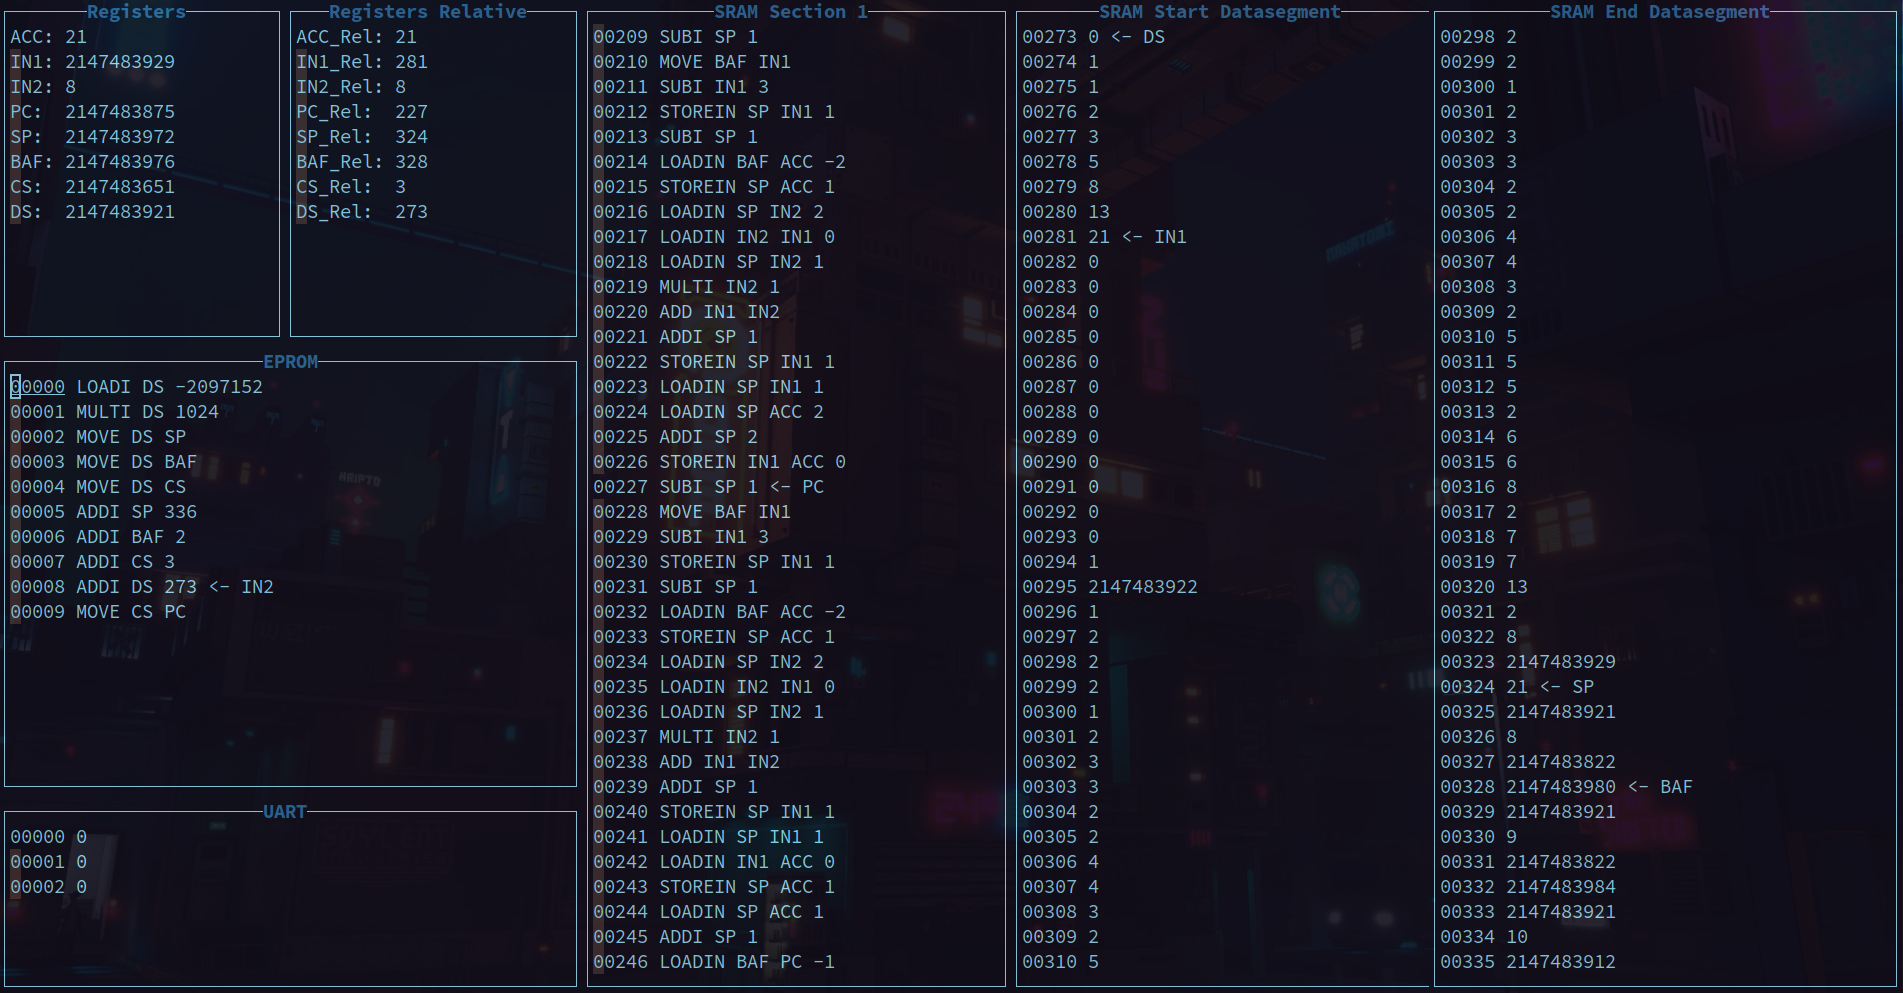
\includegraphics[width=\textwidth]{./figures/layout.png}
	\caption{Layout}
  \label{fig:layout}
\end{figure}
\begin{figure}[H]
	\begin{minipage}[b]{0.5\textwidth}
		\centering
		
\includegraphics[width=\textwidth]{./figures/input_field.png}
		\caption{Output popup}
    \label{fig:output popup}
	\end{minipage}
	\begin{minipage}[b]{0.5\textwidth}
		\centering
		
\includegraphics[width=\textwidth]{./figures/output_popup.png}
		\caption{Error popup}
    \label{fig:error popup}
	\end{minipage}
\end{figure}
\begin{figure}[H]
	\centering
	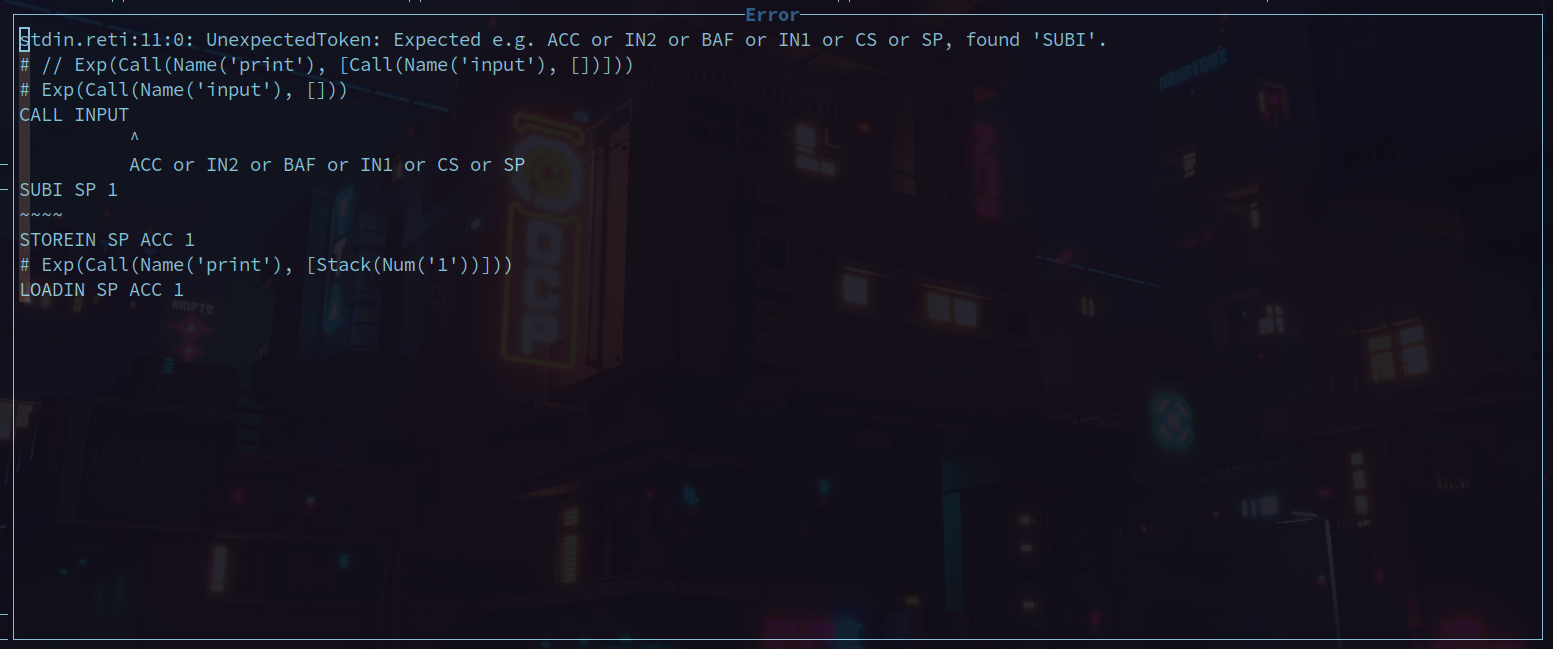
\includegraphics[width=\textwidth]{./figures/error_popup.png}
	\caption{Input field}
  \label{fig:input field}
\end{figure}
\begin{figure}[H]
	\centering
	\begin{minipage}[t]{0.49\textwidth}
		\centering
		\begin{minipage}[b]{0.35\textwidth}
			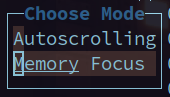
\includegraphics[width=\textwidth]{./figures/menu.png}
		\end{minipage}
		\caption{Menu to switch scrolling mode}
    \label{fig:menu}
	\end{minipage}
	\begin{minipage}[t]{0.49\textwidth}
		\centering
		\begin{minipage}[b]{0.5\textwidth}
			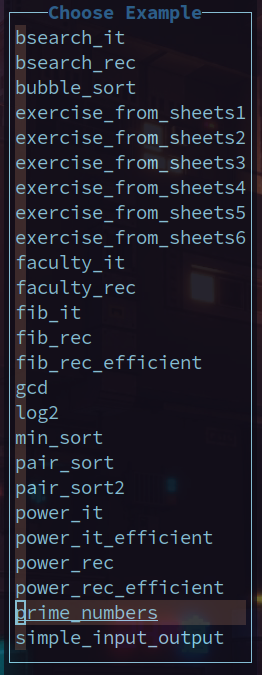
\includegraphics[width=\textwidth]{./figures/menu_example.png}
		\end{minipage}
		\caption{Menu to choose example}
    \label{fig:menu example}
	\end{minipage}
\end{figure}

\section{Properties ensured by the statemachine}
\label{sec:properties ensured by the statemachine}

In section \ref{sec:unexpected behavior} the following list of properties ensured by the statemachine for action control was mentioned. As these properties are just additional information for readers that have further interest in understanding the statemachine and they are not information relevant for understanding the RETI-Debugger, they are listed here:
\begin{itemize}
	\item If the window \alert{layout} is \alert{visible} it shouldn't be possible to load an example PicoC program via the command \inlinebox{:LoadPicoCExample}, compile one via the command \inlinebox{:CompilePicoCBuffer} or start a RETI program in the RETI-Debugger via the command \inlinebox{:StartRETIBuffer}
	\begin{itemize}
		\item This property is neccessary, because this commands and their associated actions will then be executed within a buffer of the window layout that is only supposed to hold specific window content like registers and their values or the memory cells of a specific memory and their saved values or instructions.
	\end{itemize}
	\item If the RETI-\alert{Interpreter hasn't terminated} it shouldn't be possible to start a RETI program via the command \inlinebox{:StartRETIBuffer} which would be possible if the window layout was hided
	% TODO: compiled RETi program streichen
	\begin{itemize}
		\item The property is neccessay, because else several RETI-Interpreter processes could be started and one would like to only have one RETI-Interpreter process running at a time
	\end{itemize}
	\item If a \alert{popup} window, like an input, output or error window is \alert{visible} or the RETI-\alert{Interpreter terminated} it shouldn't be possible to execute the \inlinebox{next} action
	\begin{itemize}
		\item This property is neccessary, because if the user is constantly executing the \inlinebox{next} action and a popup appears and the user is still able to continue executing the \inlinebox{next} action, then more an more popup windows could be mounted on top of each other
		\item Another reason for it being neccessary could be that, when the \inlinebox{CALL INPUT <reg>} instruction requires input, the execution of the next command could be triggered without that input could be typed in by the user. As the string \texttt{"next"} is not a valid number for the \inlinebox{CALL INPUT <reg>} instruction an exception within the RETI-Interprer will be triggered
		\item And the last reason why this property is neccessary is that, if the RETI-Interpreter terminated no next command can be executed
	\end{itemize}
	\item If a \alert{popup} window, like an input, output or error window is \alert{visible} the size of the layout shouldn't update until the popup is closed
	\begin{itemize}
		\item This property is neccessary, because of specific implementation details of the Nui library. Returning to the original buffer after focusing the popup window doesn't work if in between the size of the layout changed.
	\end{itemize}
\end{itemize}

The properties just listed are just a few examples of the properties ensured by the statemachine to give an idea. The RETI-Debugger does also have a few smaller statemachines that take care of other smaller tasks. Also explaining these smaller statemachines would be too much detail and effort for this report.

\section{Covered Topics}

In section \ref{sec:choosen_topics} the choice for the two topics from the lecture which would be covered in more detail within the main part of the report was explained and thereby the following table \ref{tab:topics}, listing all covered topics from he lecture was also referenced. As this table is excluded from counting into the page count of the main part of the report, it is included in the appendix.

\begin{table}[H]
	\centering
	\begin{tblr}{
		width = \linewidth,
		colspec = {Q[1]Q[3]},
		column{1} = {PrimaryColorDimmed, c},
		column{2} = {BoxColor, l},
		row{1} = {PrimaryColor, fg=white},
		hlines = {PrimaryColor},
		vlines = {PrimaryColor},
		}
		Topics                 & Description                                                                                                                                                                                                                                                                                          \\
		Texteditor: Vim/Neovim & {\labelitemi\hspace{\dimexpr\labelsep+0.5\tabcolsep}Creating a Neovim plugin that communicates with the RETI-Interpreter and PicoC-Compiler following a protocol to inter alia show the state of the RETI processor after each instruction and compile the PicoC code within the buffer to RETI code \\\labelitemi\hspace{\dimexpr\labelsep+0.5\tabcolsep}As fully featured IDE with language server and autoformater for lua and python by using lazy.nvim} \\
		Automation: Python     & {\labelitemi\hspace{\dimexpr\labelsep+0.5\tabcolsep}Language used in the RETI-Interpreter and PicoC-Compiler which was extended to act like a deamon that communicates with the RETI-Debugger Neovim plugin. Furthermore:                                                                            \\\hspace*{0.5\leftmargin}\labelitemii\hspace{\dimexpr\labelsep+0.5\tabcolsep}Reading metadatafrom comments was added\\\hspace*{0.5\leftmargin}\labelitemii\hspace{\dimexpr\labelsep+0.5\tabcolsep}The code quality was improved by restructering parts of the code\\\hspace*{0.5\leftmargin}\labelitemii\hspace{\dimexpr\labelsep+0.5\tabcolsep}Several bugs have been fixed}                                                                                                                                                                                                                \\
		Docker                 & {\labelitemi\hspace{\dimexpr\labelsep+0.5\tabcolsep} To provide a way for the students who are going to test this plugin to quickly set up and run the plugin with the provided \href{https://github.com/matthejue/RETI-Debugger/blob/main/Dockerfile}{Dockerfile}                                   \\\labelitemi\hspace{\dimexpr\labelsep+0.5\tabcolsep} The PDF of this report was autogenerated with the help of Github Actions with \href{https://github.com/matthejue/RETI-Debugger_Documentation/blob/master/.github/workflows/create_and_upload_pdf.yml}{this} script which is syntactically in many ways similar to Docker Compose}                                                                                                                                       \\
		% \\\labelitemi\hspace{\dimexpr\labelsep+0.5\tabcolsep} As a way to know whether the plugin also works apart of my own working environment
		% \\\labelitemi\hspace{\dimexpr\labelsep+0.5\tabcolsep} As a way to document the installation of the plugin}                                                                                                                                                                                                                                                \\
		% Linux                  & {\labelitemi\hspace{\dimexpr\labelsep+0.5\tabcolsep}I was running NixOS, a quite special linux distribution for developing the plugin, which, by it's high configurability enabled a fast workflow that wouldn't be possible in other non-linux operating systems}                                   \\
		% Git and Github         & {\labelitemi\hspace{\dimexpr\labelsep+0.5\tabcolsep}Used as version control system for the development of the RETI-Debugger Neovim Plugin and PicoC-Compiler and RETI-Interpreter                                                                                                                    \\\labelitemi\hspace{\dimexpr\labelsep+0.5\tabcolsep}Github was used as place from which both the PicoC-Compiler and RETI-Interpreter executable and also the RETI-Debuger Neovim plugin get downloaded using lazy.nvim} \\
		Latex                  & {\labelitemi\hspace{\dimexpr\labelsep+0.5\tabcolsep}Used for writing this report and thus also the documentation for the RETI-Debugger Neovim plugin in the appendix of this report                                                                                                                  \\\labelitemi\hspace{\dimexpr\labelsep+0.5\tabcolsep}Used for writing a template used in this report that is also going to be used in my master thesis}\\
		% LLM's                  & {\labelitemi\hspace{\dimexpr\labelsep+0.5\tabcolsep}I used \url{https://www.perplexity.ai/} a lot to quickly get answers to some questions about lua, python, latex and certain \inlinebox{vim.loop} (i.e. libuv), \inlinebox{vim.api} functions} and vim settings                                   \\
	\end{tblr}
	\caption{Topics covered in the project}
	\label{tab:topics}
\end{table}

\chapter{Bibliography}
\printbibliography[heading=none]

\end{document}

% Fleury: Da ja eigenes Template
% brauchen wir Abstract oder so wie in Example PDF?
% Schtiftgröße in Bildern ok?
% zählt Titel auch in Seitenzahl rein?
% Transitions so ok?

% Latex Sourcecode selbst explizit verlinken. Unterscheidung zwischen PDF und Sourcecode
